%====================================================================================
\section{Análisis de las series}
%====================================================================================

\begin{frame}{Análisis de las series}
	\begin{itemize}
		\item La mayoría de series de tiempo económicas se caracterizan por estar compuestas por una tendencia, un comportamiento estacional y un componente irregular:
			$$y = \text{tendencia} + \text{estacional} + \text{irregular}$$
		\item Luego de quitar las dos primeras, el problema se reduce a modelar el comportamiento irregular, que puede ser ``estacionario'' o contener al menos una ``raíz unitaria''.
	\end{itemize}
\end{frame}
%---------------------------------------------------
\begin{frame}{Estudiando el componente irregular. Procesos Estocásticos Estacionarios}
	\begin{itemize}
		\item  Una serie se define como estacionaria si los momentos de primer y segundo orden de dicho proceso estocástico son invariantes en el tiempo.
		\item Estos momentos incluyen la esperanza (media) y varianza de la serie, pero también las covarianzas y correlaciones entre los valores rezagados de la misma.
	\end{itemize}
\end{frame}
%---------------------------------------------------
\begin{frame}{Estudiando el componente irregular. Procesos Estocásticos No Estacionarios (Raíz unitaria)}
	\begin{itemize}
		\item En el caso de las series estacionarias estas tienen la característica de que sus valores oscilan alrededor de la media. Así, si una variable se desvía del valor de su media existen fuerzas que hacen que la serie retorne a su media. \textcolor{red}{La estacionariedad nos dice que el pasado es relevante!}
		\item El caso de la raíz unitaria es totalmente opuesto: los shocks que puedan afectar a la serie en determinado momento la desviarán por un lapso indeterminado de su valor medio. Por ello se dice que estos procesos tienen memoria larga y la serie deambula alrededor de su media. \textcolor{red}{La presencia de raíz unitaria significa que la serie no puede ser predicha usando su pasado}
	\end{itemize}
\end{frame}
%---------------------------------------------------
\begin{frame}{Serie estacionaria y no estacionaria}
	\centering
		\begin{figure}
			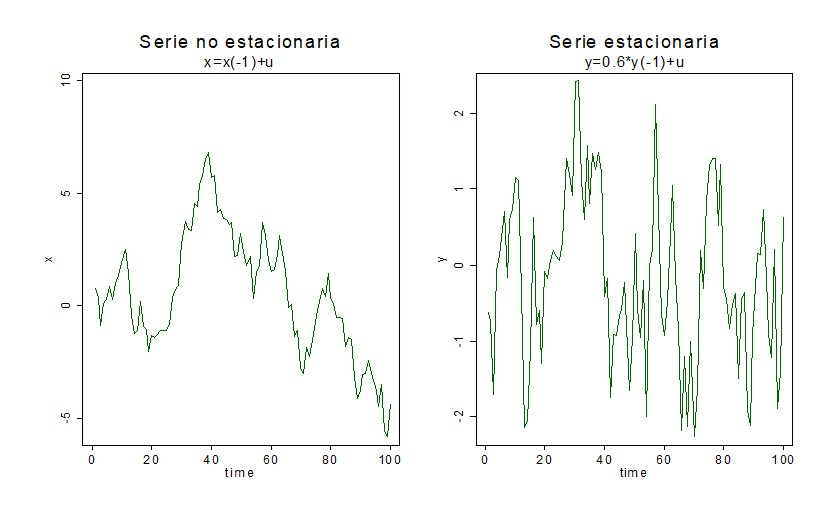
\includegraphics[width = 0.9\linewidth]{fig/figure3.jpg}
		\end{figure}
\end{frame}
%---------------------------------------------------
\begin{frame}{Descomposición de series}
	\begin{itemize}
		\item Sobre una serie temporal \textbf{$Y_t$} podemos identificar una serie de componentes básicos que se denominan respectivamente como:
		\item \textbf{TENDENCIA}: Movimientos de larga duración que se mantienen durante todo el periodo de observación.
		\item \textbf{ESTACIONALIDAD}: Movimiento que se produce, dentro de un periodo anual, por motivos no estrictamente económicos  como climáticos.
		\item \textbf{IRREGULARIDAD}: Movimientos erráticos que pueden o no ser predichos dependiendo de la característica de esta.
	\end{itemize}
\end{frame}
%---------------------------------------------------
\begin{frame}
	\centering
		\begin{figure}
			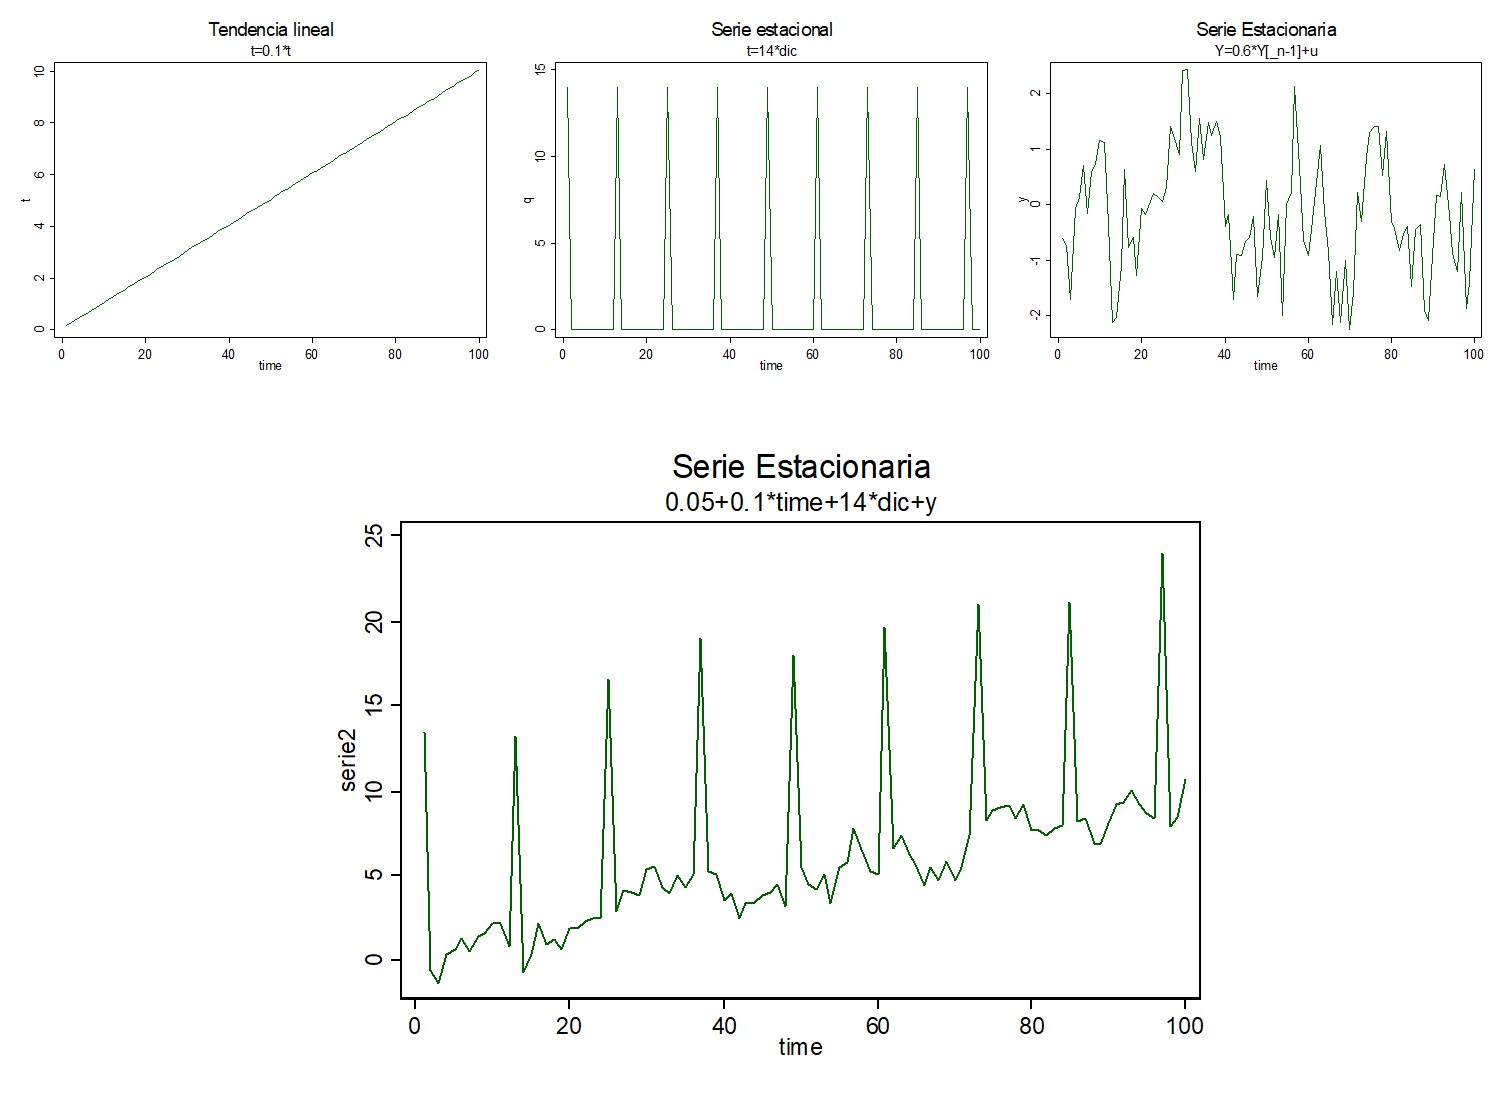
\includegraphics[width = 0.9\linewidth]{fig/figure4.jpg}
		\end{figure}
\end{frame}
